\documentclass[11pt,twocolumn]{article}
\usepackage{fullpage}
\usepackage{graphicx}
\usepackage{subcaption}
\usepackage{todonotes}
\usepackage{listings}
\usepackage{hyperref}
\lstset{language=Python}

\newcommand{\TODO}[1]{\todo[inline]{#1}}

\newcommand{\TITLE}{MLCommons Earthquake Benchmark}
\newcommand{\AUTHOR}{Gregor von Laszewski, Jacques Fleischer, Geoffrey C. Fox}

\title{\TITLE}
\author{\AUTHOR}


\begin{document}
\onecolumn
\begin{center}
{\huge \TITLE}

{\AUTHOR}
\end{center}

\tableofcontents
\twocolumn


\maketitle

\begin{abstract}

  We report here the results of the MLCommons Science Working group benchmark of the Earthquake code.

\end{abstract}

\section{Setup}

The code is relatively easy to set up for use on various computers
using NVIDIA Cards. The code has been run on A100, V100, K100, P100,
and RTX3090. Other cards may be also supported, but the code requires
a fair amount of memory. Therefore, it may not be able to be run on
NVIDIA Cards with less than 24GB of memory.

The documentation on how to set up the code is available as part of a
\href{https://github.com/laszewsk/mlcommons/tree/main/benchmarks/earthquake#readme}{README.md}
file~\cite{www-earthquake-setup}.


\section{Cloudmesh}

The code has been enhanced with benchmark functions from Cloudmesh~\cite{www-cloudmesh}.
It also uses a convenient extension to batch scripts called
cloudmesh-sbatch allowing more easily to place additional templated
parameters into the SBATCH or LSF shell script parameters when
submitting to batch systems. In addition, we have developed a cloudmesh
compute cluster workflow management tool that allows us to submit the
codes in parallel to multiple supercomputers as well as parallel batch
jobs~\cite{las-cc,las21openapi}


\TODO{2 Week Intervals is the wrong label, label must be unique}  


\section{Benchmark Terminology}

\begin{tabular}{rl}
NNSE & 2 Week Intervals \\
\hline
Year Back & % describe each one of these values \\
2wk+7AVG & The average of 7 two-week intervals \\
2wk+13AVG & The average of 13 two-week intervals \\
6 Months Back & \\
2wk+13AVG & \\
3 Months Back & \\
2wk+7AVG & \\
2wk+7AVG & \\
2wk+26AVG & \\
2wk+26AVG & \\
2wk+13AVG & \\
2wk+26AVG & \\
2wk+7AVG & \\
2wk+13AVG & \\
2 weeks Now & \\
2wk+26AVG & \\
\hline
\end{tabular}

\section{Results from Rivanna V100}

Rivanna is a supercomputer located at the University
of Virginia. It has a variety of CUDA cards, including
an A100, V100, K80. In this benchmark we use its V100.

\subsection{Best Accuracy}

Just one entry for best accuracy.

\subsection{Accuracy Comparison}

We compare accuracy.

\subsection{Time Comparison}

We compare time.

\subsection{Power Consumption}

We compare power.


\begin{figure*}[p]
     \centering
     \begin{subfigure}[b]{0.49\textwidth}
        \centering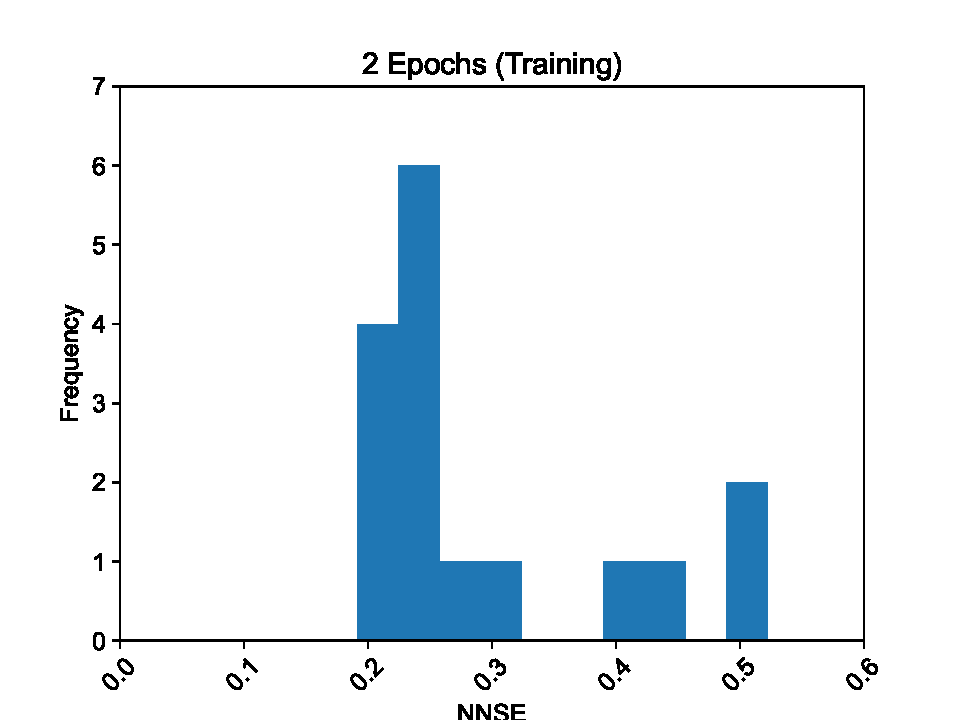
\includegraphics[width=1.0\linewidth]{images/2_training-NNSE.pdf}
        \caption{NNSE - 2 epochs}
        \label{fig:tbd1}
     \end{subfigure}
     \hfill
     \begin{subfigure}[b]{0.49\textwidth}
        \centering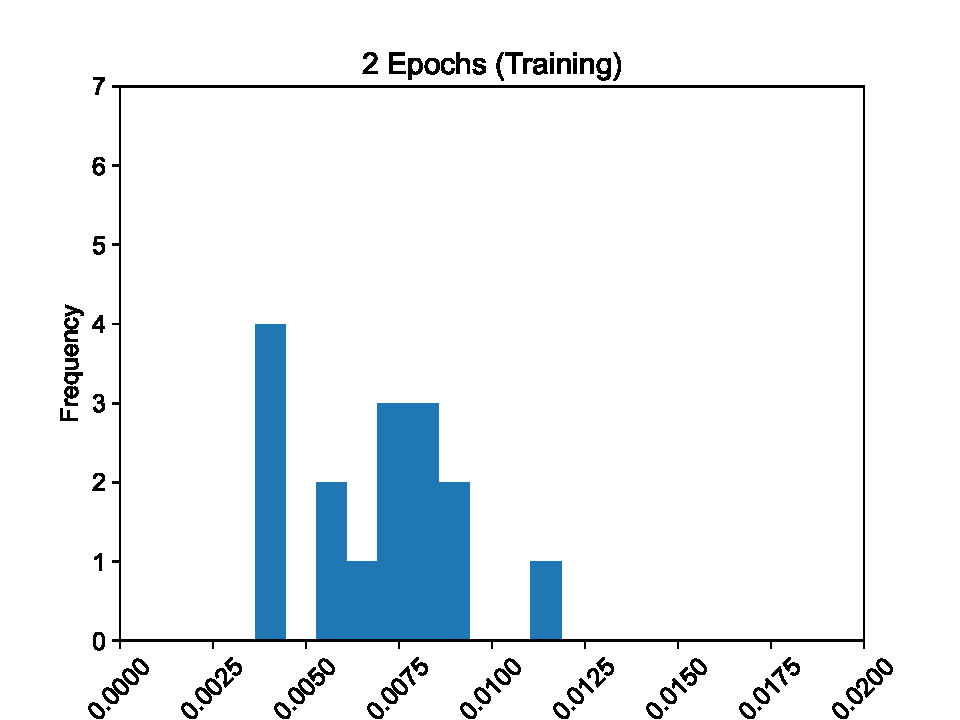
\includegraphics[width=1.0\linewidth]{images/2_training-MSE.pdf}
        \caption{MSE - 2 epochs}
        \label{fig:tbd2}
     \end{subfigure}
     \hfill
     \newline
     \begin{subfigure}[b]{0.49\textwidth}
        \centering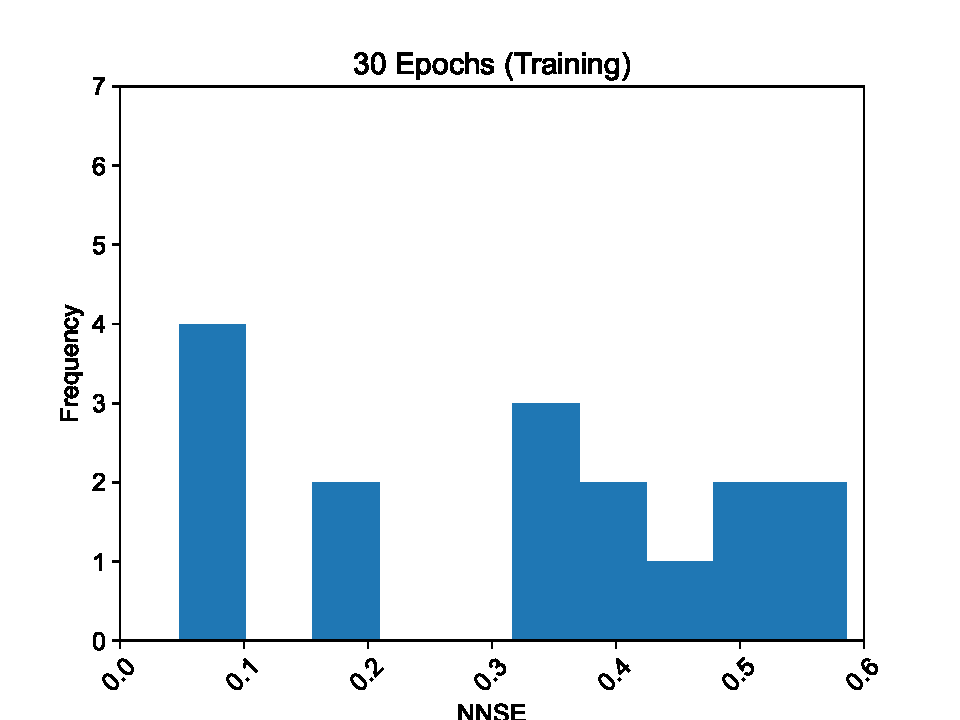
\includegraphics[width=1.0\linewidth]{images/30_training-NNSE.pdf}
        \caption{NNSE - 30 epochs}
        \label{fig:tbd3}
     \end{subfigure}
     \hfill
     \begin{subfigure}[b]{0.49\textwidth}
        \centering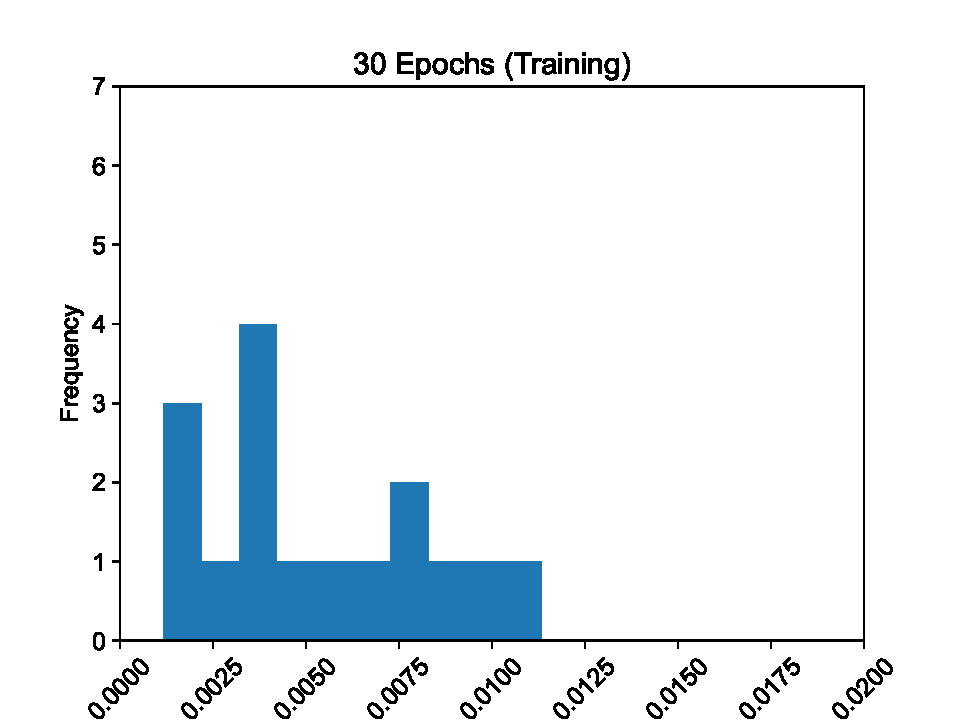
\includegraphics[width=1.0\linewidth]{images/30_training-MSE.pdf}
        \caption{MSE - 30 epochs}
        \label{fig:tbd4}
     \end{subfigure}
     \hfill
          \newline
     \hfill
     \begin{subfigure}[b]{0.49\textwidth}
        \centering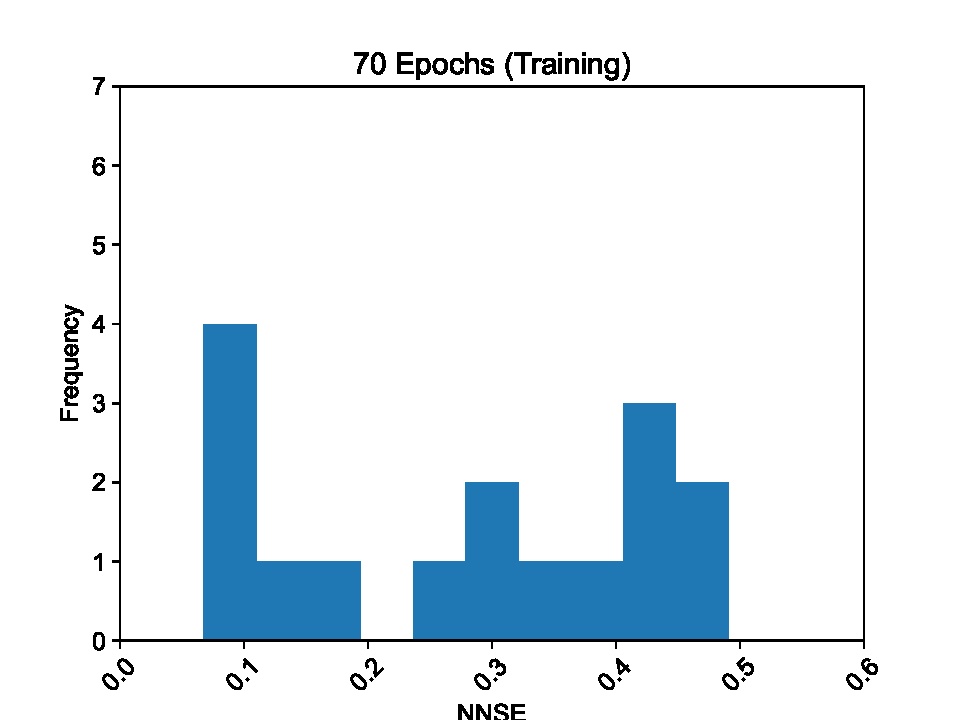
\includegraphics[width=1.0\linewidth]{images/70_training-NNSE.pdf}
        \caption{NNSE - 70 epochs}
        \label{fig:tbd3}
     \end{subfigure}
     \hfill
     \begin{subfigure}[b]{0.49\textwidth}
        \centering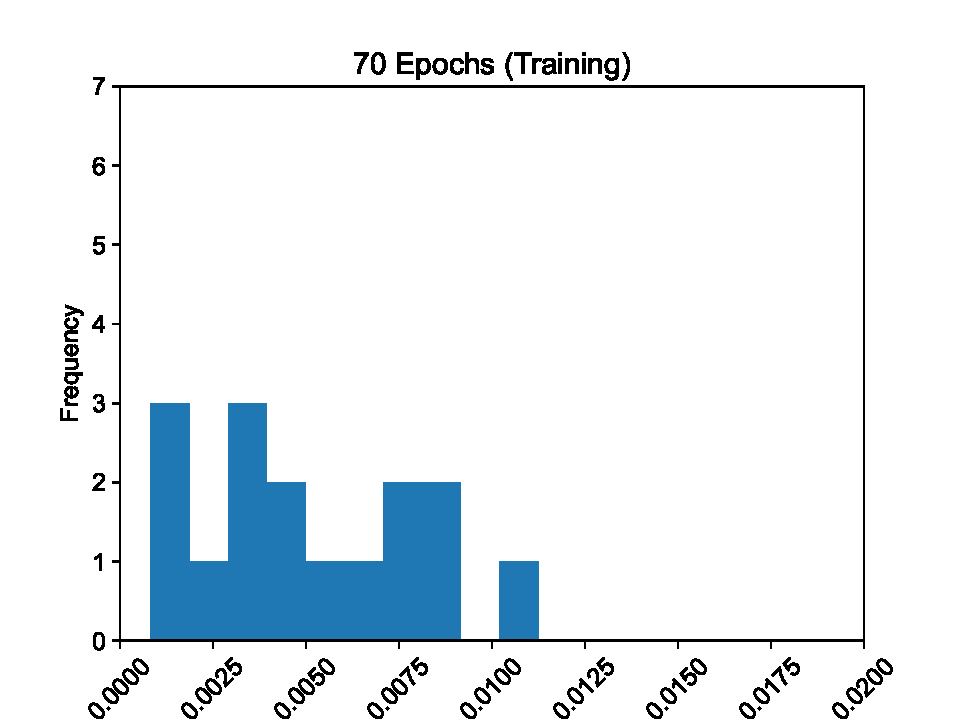
\includegraphics[width=1.0\linewidth]{images/70_training-MSE.pdf}
        \caption{MSE - 70 epochs}
        \label{fig:tbd4}
     \end{subfigure}
        \caption{NNSE and MSE values for epochs 2, 30, 70 (training).}
        \label{fig:six graphs}
\end{figure*}

\begin{figure*}[p]
     \centering
     \begin{subfigure}[b]{0.49\textwidth}
        \centering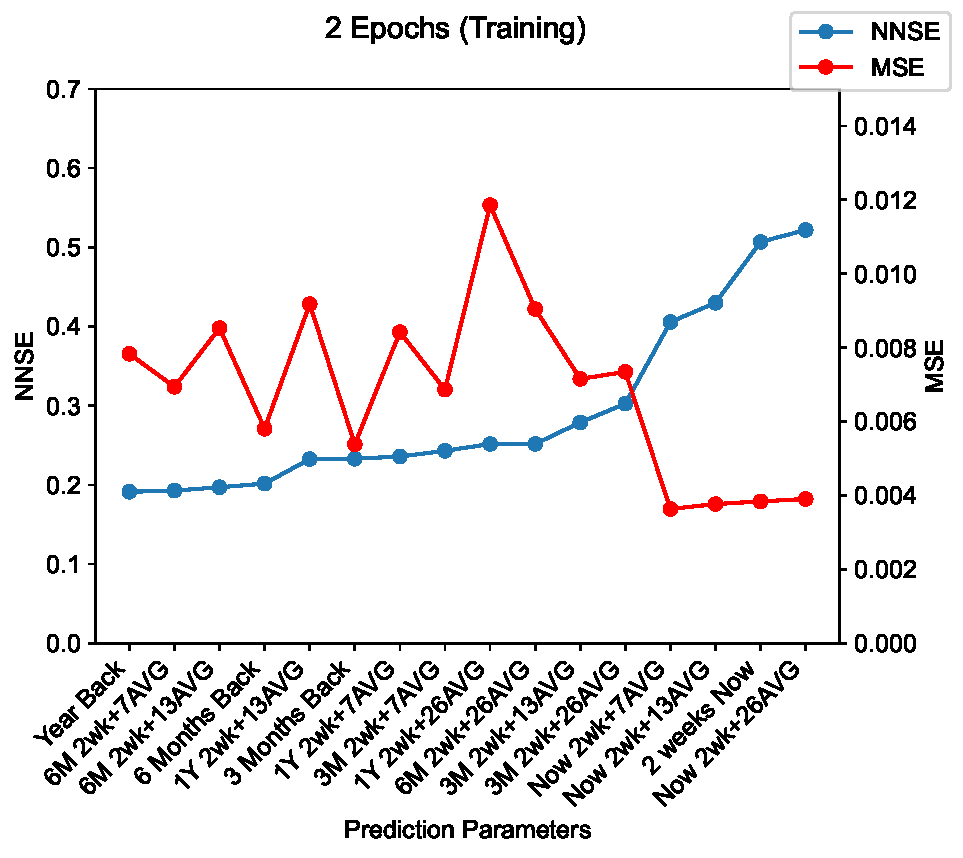
\includegraphics[width=1.0\linewidth]{images/2_training-MSE-and-NNSE.pdf}
        \caption{MSE and NNSE - 2 epochs training}
        \label{fig:tbd1}
     \end{subfigure}
     \hfill
     \begin{subfigure}[b]{0.49\textwidth}
        \centering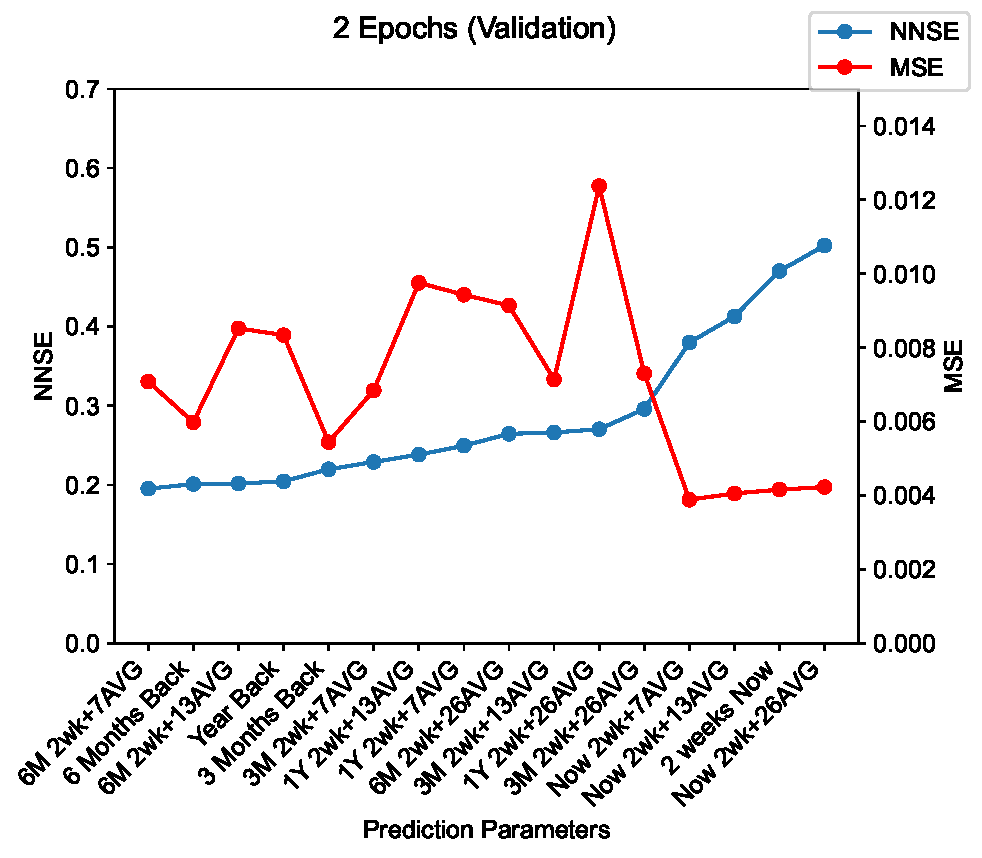
\includegraphics[width=1.0\linewidth]{images/2_validation-MSE-and-NNSE.pdf}
        \caption{MSE and NNSE - 2 epochs validation}
        \label{fig:tbd2}
     \end{subfigure}
     \hfill
     \newline
     \begin{subfigure}[b]{0.49\textwidth}
        \centering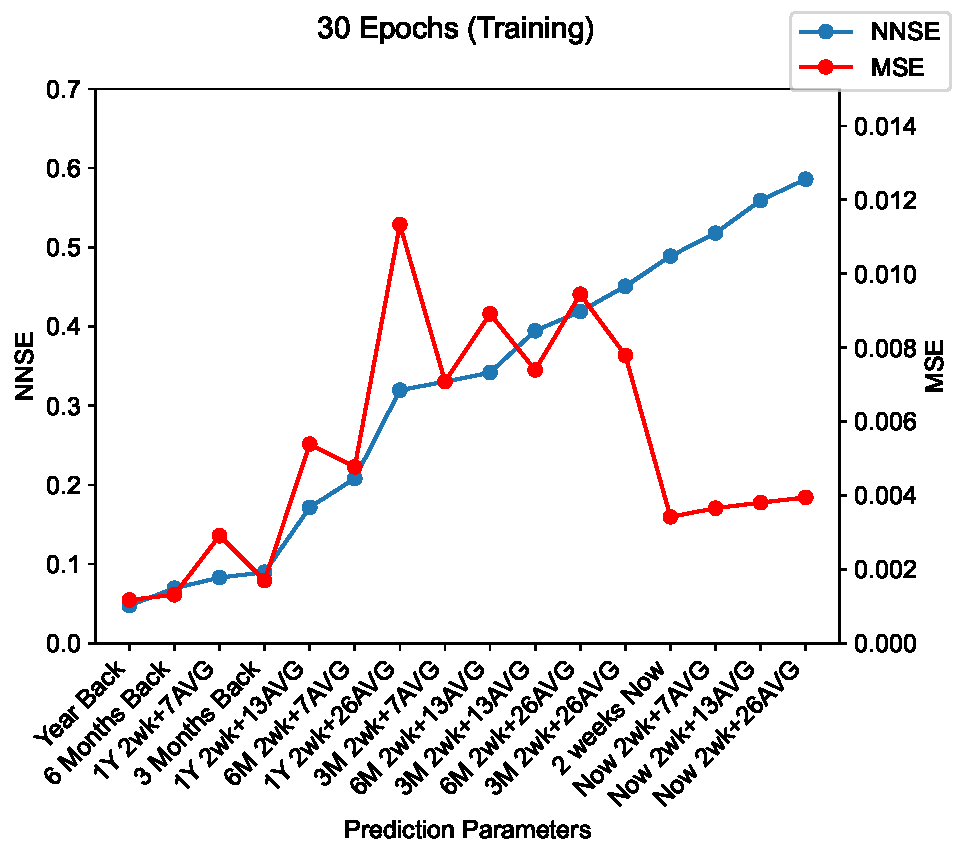
\includegraphics[width=1.0\linewidth]{images/30_training-MSE-and-NNSE.pdf}
        \caption{MSE and NNSE - 30 epochs training}
        \label{fig:tbd3}
     \end{subfigure}
     \hfill
     \begin{subfigure}[b]{0.49\textwidth}
        \centering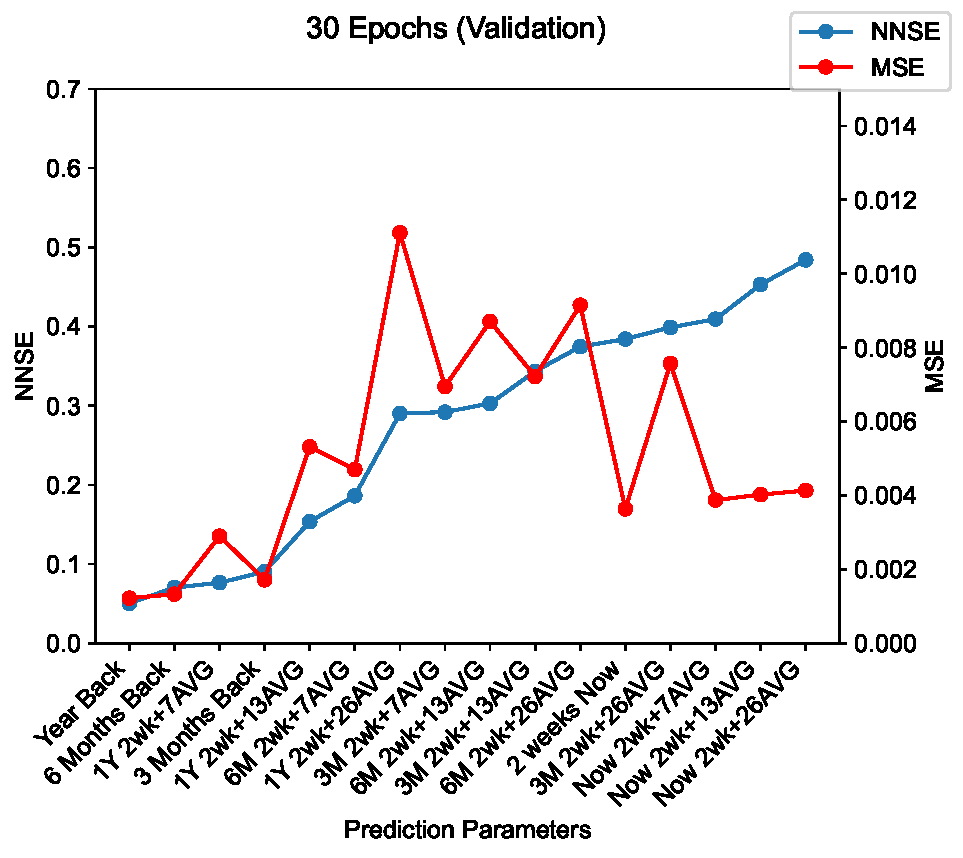
\includegraphics[width=1.0\linewidth]{images/30_validation-MSE-and-NNSE.pdf}
        \caption{MSE and NNSE - 30 epochs validation}
        \label{fig:tbd4}
     \end{subfigure}
     \hfill
          \newline
     \hfill
     \begin{subfigure}[b]{0.49\textwidth}
        \centering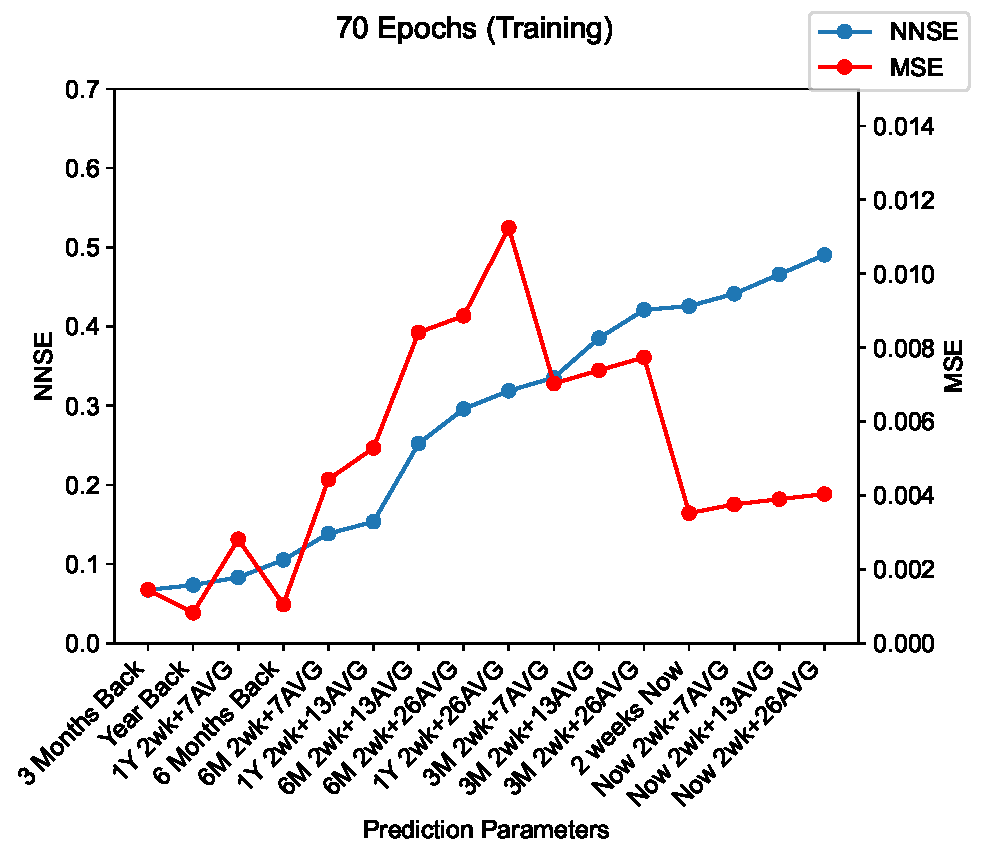
\includegraphics[width=1.0\linewidth]{images/70_training-MSE-and-NNSE.pdf}
        \caption{MSE and NNSE - 70 epochs training}
        \label{fig:tbd3}
     \end{subfigure}
     \hfill
     \begin{subfigure}[b]{0.49\textwidth}
        \centering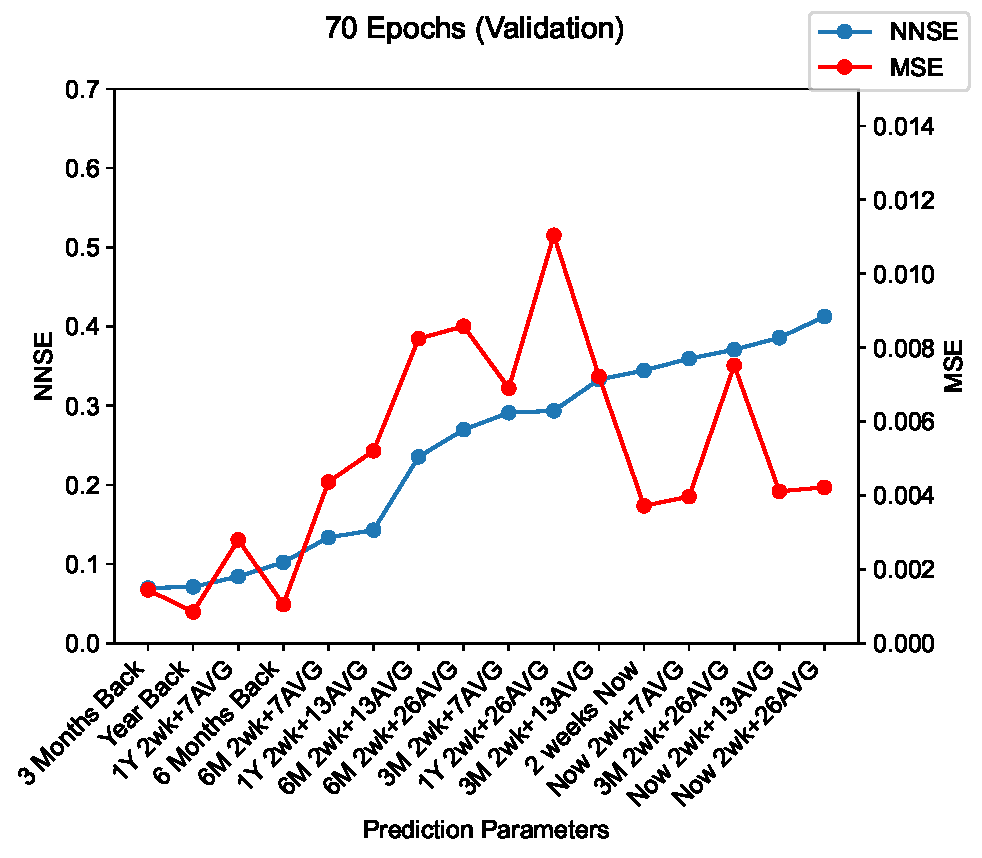
\includegraphics[width=1.0\linewidth]{images/70_validation-MSE-and-NNSE.pdf}
        \caption{MSE and NNSE - 70 epochs validation}
        \label{fig:tbd4}
     \end{subfigure}
        \caption{NNSE and MSE values for epochs 2, 30, 70 (training and validation).}
        \label{fig:six graphs}
\end{figure*}

\begin{figure}[htb]
%\centering\includegraphics[width=1.0\columnwidth]{usecase/images/hvac-new-arch.png}
\centering\includegraphics[width=1.0\columnwidth]{images/2-weeks-now.pdf}
\caption{To be determined}
\label{fig:tbd}
\end{figure}

\begin{table}[htb]
%\centering\includegraphics[width=1.0\columnwidth]{usecase/images/hvac-new-arch.png}

\caption{To be determined}
\label{tab:tbd}
\bigskip
%\resizebox{1.0\columnwidth}{!}{%
\centering\begin{tabular}{rl}
NNSE & name \\
\hline
0.191300 & Year Back \\
0.192700 & 6M 2wk+7AVG \\
0.197000 & 6M 2wk+13AVG \\
0.201600 & 6 Months Back \\
0.232600 & 1Y 2wk+13AVG \\
0.233000 & 3 Months Back \\
0.235800 & 1Y 2wk+7AVG \\
0.243000 & 3M 2wk+7AVG \\
0.251600 & 1Y 2wk+26AVG \\
0.251700 & 6M 2wk+26AVG \\
0.278800 & 3M 2wk+13AVG \\
0.302500 & 3M 2wk+26AVG \\
0.405600 & Now 2wk+7AVG \\
0.429900 & Now 2wk+13AVG \\
0.506800 & 2 weeks Now \\
0.521800 & Now 2wk+26AVG \\
\hline
\end{tabular}%
%}
\end{table}

\begin{table}[htb]
%\centering\includegraphics[width=1.0\columnwidth]{usecase/images/hvac-new-arch.png}

\caption{To be determined}
\label{tab:tbdetermined}
\bigskip
%\resizebox{1.0\columnwidth}{!}{%
\centering\begin{tabular}{rl}
NNSE & 2 Week Intervals \\
\hline
0.195200 & 6M 2wk+7AVG \\
0.201000 & 6 Months Back \\
0.201600 & 6M 2wk+13AVG \\
0.204500 & Year Back \\
0.219700 & 3 Months Back \\
0.228900 & 3M 2wk+7AVG \\
0.238200 & 1Y 2wk+13AVG \\
0.249500 & 1Y 2wk+7AVG \\
0.264400 & 6M 2wk+26AVG \\
0.266200 & 3M 2wk+13AVG \\
0.270300 & 1Y 2wk+26AVG \\
0.295800 & 3M 2wk+26AVG \\
0.379700 & Now 2wk+7AVG \\
0.412700 & Now 2wk+13AVG \\
0.470100 & 2 weeks Now \\
0.502300 & Now 2wk+26AVG \\
\hline
\end{tabular}%
%}
\end{table}

\section*{Acknowledgements}

Continued work was in part funded by the NSF CyberTrain-
ing: CIC: CyberTraining for Students and Technologies from
Generation Z with the award numbers 1829704 and 2200409
and NIST 60NANB21D151T.


\bibliographystyle{IEEEtran}
\bibliography{report}


\end{document}
